%!TEX root = ../main.tex

\section*{Results}

  \subsection*{\acl{micone} (\acs{micone})}

  We have developed \ac{micone}, a flexible and modular pipeline for 16S amplicon sequencing rRNA data (hereafter mentioned simply as 16S data) analysis, that allows us to infer microbial co-occurence networks.
  It incorporates various popular, publicly available tools as well as custom Python modules and scripts to facilitate inference of co-occurrence networks from 16S data. Using \ac{micone} one can obtain co-occurrence networks by applying to 16S data (or to already processed taxonomic count matrices) any combination of the available tools. The effects of changing any of the intermediate step can be monitored and evaluated in terms of its final network outcome, as well as on any of the intermediate metrics and data outputs.
  The \ac{micone} pipeline workflow is shown in Figure~\ref{fig:figure1}.
  The different steps for going from 16S data to co-occurrence networks can be grouped into four major modules; (i) the denoising and clustering (DC) step, which handles denoising of the raw 16S sequencing data into representative sequences; (ii) the taxonomy assignment (TA) step that assigns taxonomic labels to the representative sequences; (iii) the OTU processing (OP) step that filters and transforms the taxonomy abundance table; and finally (iv) the network inferences (NI) step which infers the microbial co-occurrence network.
  Each process in the pipeline supports alternate tools for performing the same task (see Methods and Figure~\ref{fig:figure1}). A centralized configuration file contains all the specifications for what modules to be used in the pipeline, and can be modified by the user to choose the desired set of tools.
  In what follows, we perform a systematic analysis of each step of the pipeline to estimate how much the final co-occurrence network depends on the possible choices at each step. We also evaluate a large number of tool combinations to determine a set of recommended default options for the pipeline and provide the users with a set of guidelines to facilitate tool selection as appropriate for their data.

  \begin{figure}[h]
    \centering
    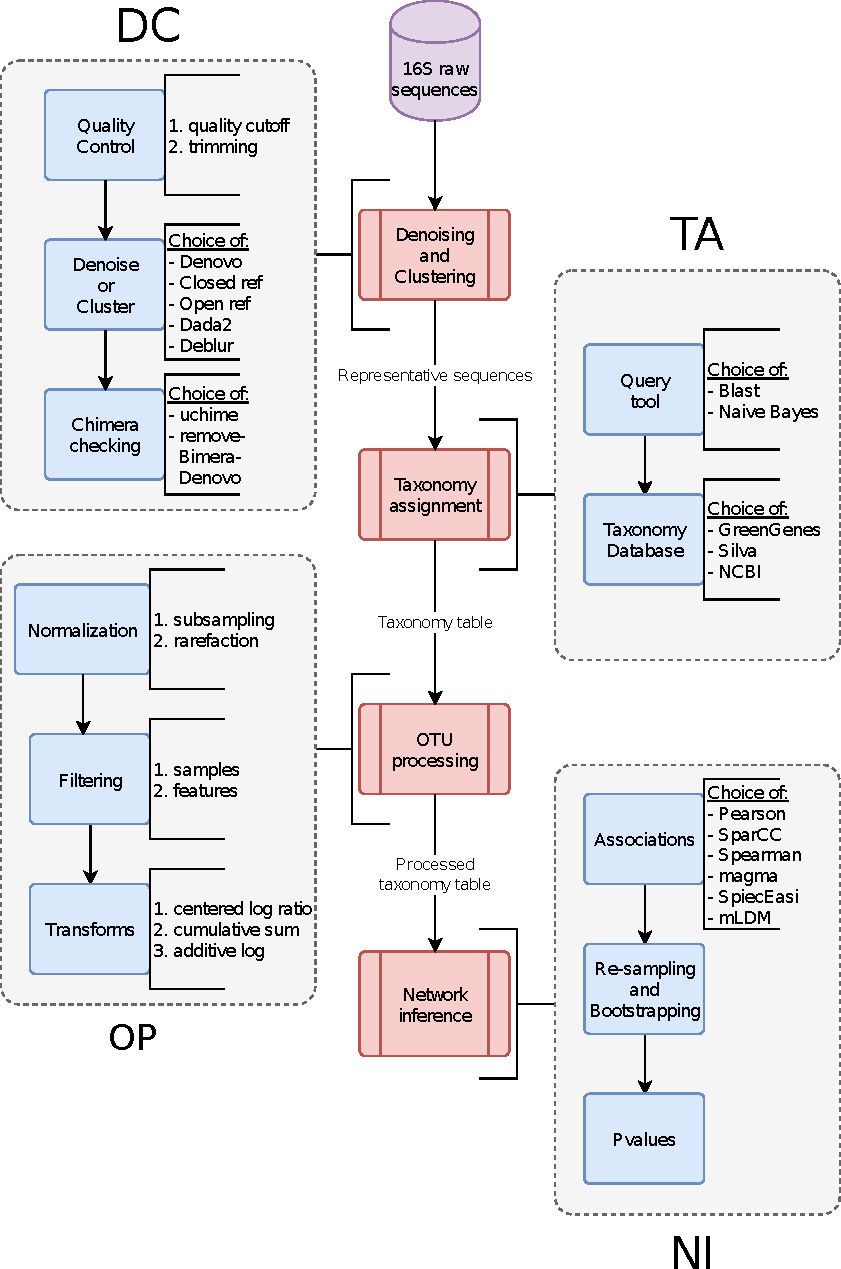
\includegraphics[width=0.69\linewidth]{figure1.pdf}
    \caption{
      \textbf{The workflow of the microbial co-occurrence analysis pipeline}.
      The processes can be grouped into four major steps: \textbf{(DC)} denoising and clustering, \textbf{(TA)} taxonomy assignment, \textbf{(OP)} OTU/ESV processing, and \textbf{(NI)} network inference.
      Each step incorporates several processes, each of which in turn have several alternate algorithms for the same task (indicated by the text to the right of the blue boxes).
      The text along the arrows describes the data that is being passed from one step to another. For details on each process and data types, see Methods.
    }
    \label{fig:figure1}
  \end{figure}

  % TODO: Talk about the datasets: real, mock and synthetic (with references)
  In addition to the algorithmic pipeline itself, our analysis involves two types of data: The first type consists of sets of 16S sequencing data for real communities (see Methods). The second are datasets artificially created for the specific goal of helping evaluate computational analysis tools. In particular, in order to objectively compare, to the extent possible, how well each step in \ac{micone} best captures the underlying data, we use both mock data from mockrobiota~\cite{Bokulich2016} as well as, synthetically generated reads from an Illumina read simulator called ART~\cite{Huang2012}.
  The mock datasets selected were labelled mock4, mock12 and mock16 in the mockrobiota database and consist of sequenced 16S data from mock communities of various bacteria.
  These datasets were selected since they contained the expected compositions along with the reference sequences for the organisms in the mock community.
  The synthetic reads were simulated using the three different taxonomy distribution profiles obtained from soil, water and healthy stool microbiome datasets \hl{[refs]}.
  Reference sequences were generated using \ac{ncbi} and the Decard tool \cite{Golob2017} for these taxonomy profiles.
  Detailed information on the mock communities and the settings used to generate the synthetic data are provided in the Methods section.


  \FloatBarrier

  \subsection*{The choice of reference database has the biggest impact on inferred networks}

  % TODO: Summarized sections
  In order to analyze the effect of different statistical methods on the inferred co-occurrence networks, we generated co-occurrence networks using all possible combinations of methods and estimated the variability in the networks due to each choice.
  This analysis is performed while keeping the network inference algorithm (NI step) the same throughout the analysis.
  The effects of various steps on the final co-occurrence network is estimated by building a linear model of the edges of the network as a function the various step in the analysis pipeline (see Methods).
  Figure \ref{fig:figure2}B, shows the fraction of total variation among the co-occurrence networks as contributed by the first three steps of the pipeline. In other words, each point corresponds to a different combination of tools, and captures how much the final network is affected by such choice.
  The 16S reference database contributes the most ($\sim25\%$) to variation in the networks. This is also reflected in the fact that the networks can be clearly separated based on the database used (Figure \ref{fig:figure2}B).
  This indicates that the taxonomy assigned to the reference sequences drastically alters the co-occurrence network and this change is much more significant than how the reference sequences themselves are identified (in the DC step).
  We believe that the grouping by taxonomy assignment into clusters (..... in Fig. XXX) is due to the mislabelling of constitutive taxa that are present in high abundance in the community.
  The residual variation can be seen as an artifact that arises due to the effect on the resultant network when multiple steps are changed at the same time.
  Another interesting observation is that the dissimilarity between the networks decreases when the low abundance \ac{otu}s are removed from the network. This is visible in terms of ...
  These results enable us to believe that the most important criterion for accurate comparative analyses of co-occurrence networks is the taxonomy reference database.

  \begin{figure}[H]
    \centering
    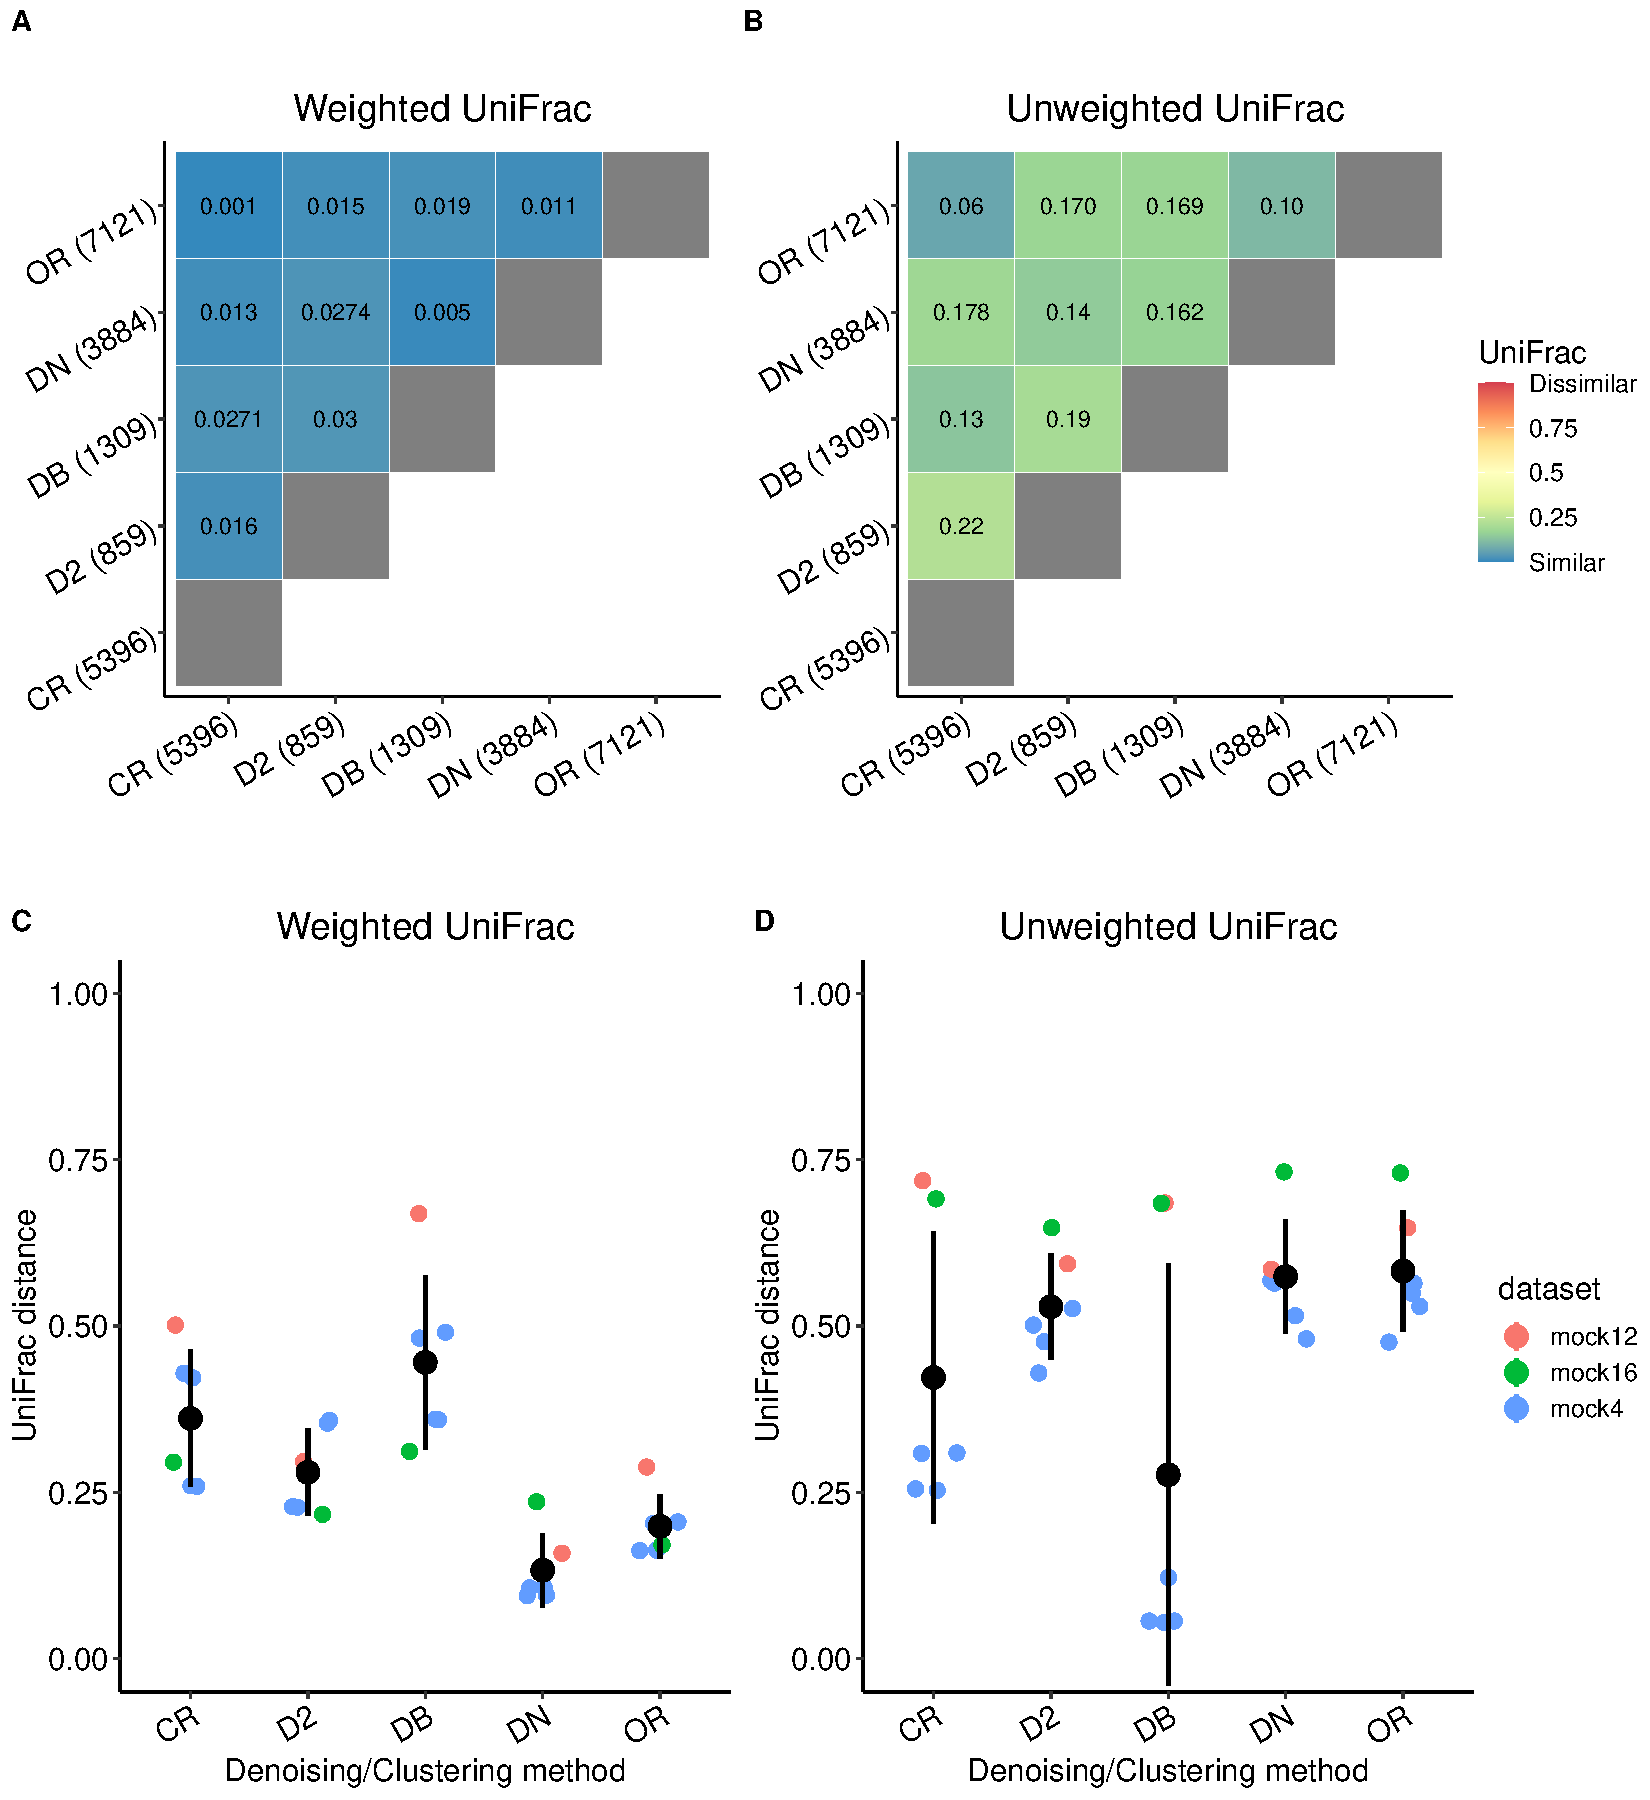
\includegraphics[width=0.85\linewidth]{figure2.pdf}
  \end{figure}
  \begin{figure}[!t]
    \centering
      \caption{
      \textbf{The choice of database contributes to the most variance in the networks}.
      \textbf{(A)} The total relative variance in the networks contributed by the DC, TA and OP steps of the pipeline (right) and the linear model used to calculate the relative variance (left).
      \textbf{(B)} All combinations of inferred networks are shown as points on a PCA plot.
      The color of the points corresponds to the taxonomy database, the shape corresponds to the denoising/clustering method and the size corresponds to whether low abundance OTUs were removed or not.
      \textbf{(B inset)} The network generated using DC=dada2, TA=GG, OP=no and NI=SPARCC and represents the particular point shown (big red square).
      The plot clearly shows that the points can be separated based on the TA step and that the differences due to the DC and OP steps are not as significant.
    }
    \label{fig:figure2}
  \end{figure}


  \FloatBarrier

  \subsection*{Denoising and clustering methods differ in their identification of less common reference sequences}

  Denoising and clustering are commonly carried out to generate representative sequences from the raw 16S sequencing data and to obtain the \ac{otu}/\ac{esv} tables (counts of these representative sequences for each sample).
  In order to compare the \ac{otu} tables generated by different tools we processed the same 16S sequencing reads (healthy samples from a fecal microbiome transplant study~\cite{Kang2017}) using 5 different methods:  open-reference clustering, closed-reference clustering, denovo clustering, \ac{dada2}~\cite{Callahan2016} and Deblur~\cite{Amir2017}.
  The first three methods are from the \ac{qiime1}~\cite{Caporaso2010} package.
  We find that there is good agreement in the \ac{otu}/\ac{esv} tables when different combinations of methods are used to generate them (Supplementary Figure~\ref{fig:figureS1}).

  To compare the representative sequences generated by these methods we employ both the weighted~\cite{Lozupone2007} (Figure~\ref{fig:figure3}A) and unweighted UniFrac method~\cite{Lozupone2005} (Figure~\ref{fig:figure3}B).
  The weighted UniFrac distance metric takes into account the counts of the representative sequences, whereas the unweighted UniFrac distance metric does not and hence gives equal weights to each sequence.
  From Figure~\ref{fig:figure3}A one can see that the representative sequences generated by the different methods are similar to each other when weighted by their abundance.
  Figure~\ref{fig:figure3}B on the other hand shows an increase in dissimilarity between each pair of methods suggesting that the methods might differ in the treatment of sequences of low abundance.
  In order to verify this claim, for each of these methods we use the \ac{gg} taxonomy database to assign taxonomies to the representative sequences.
  We then correlate the abundances of matching taxonomies between a pair of DC methods (Figure \ref{fig:figureS1}A and B).
  The \ac{esv} tables generated by methods that perform denoising are very similar to each other $\sim0.91$ and the \ac{otu} tables generated by the clustering methods are very similar to each other $\sim0.9$, but results of denoising and clustering are highly uncorrelated with each other $\sim0.4$ (Figure \ref{fig:figureS1}C).

  These comparisons only elucidate the pairwise similarity or dissimilarity of a pair of methods.
  In order to determine the tool that most accurately recapitulates the reference sequences in the samples, we use the 16S sequences from the mock datasets.
  In particular, we used the pipeline to process mock community datasets using each of the possible methods included for this step. We next compared predicted representative sequences with expected representative sequences and their distribution.
  The results (Figure~\ref{fig:figure3}C and D) show that, for the mock datasets, the different methods perform similar to each other, exactly as observed in the case of the real dataset. However, the mock predicted sequence distributions are substantially different from the expected sequence distribution.
  This result is more exaggerated in the case of the unweighted UniFrac metric, where some of the datasets show a very high deviation from the expected sequences.
  These high deviations are primarily in two of the three datasets that were analyzed and show that the datasets themselves play a big role in the performance of these methods.
  This can be clearly seen in the performance (weighted UniFrac distance) of \ac{dada2} and Deblur on mock12 and mock16 datasets, where, Deblur outperforms \ac{dada2} on mock12 but the under-performs on mock16.

  There is no method that clearly outperforms the rest in all datasets.
  Based on their slightly better performance on the mock datasets, their \textit{de novo} error correcting nature and other previous studies [refs], \ac{dada2} and Deblur seem to be in general the most reliable.
  Given the unexpected poor performance of Deblur on the synthetic data, the default algorithm in the pipeline was chosen to be \ac{dada2} (Supplementary Figure~\ref{fig:figureS3}).

  \begin{figure}
    \centering
    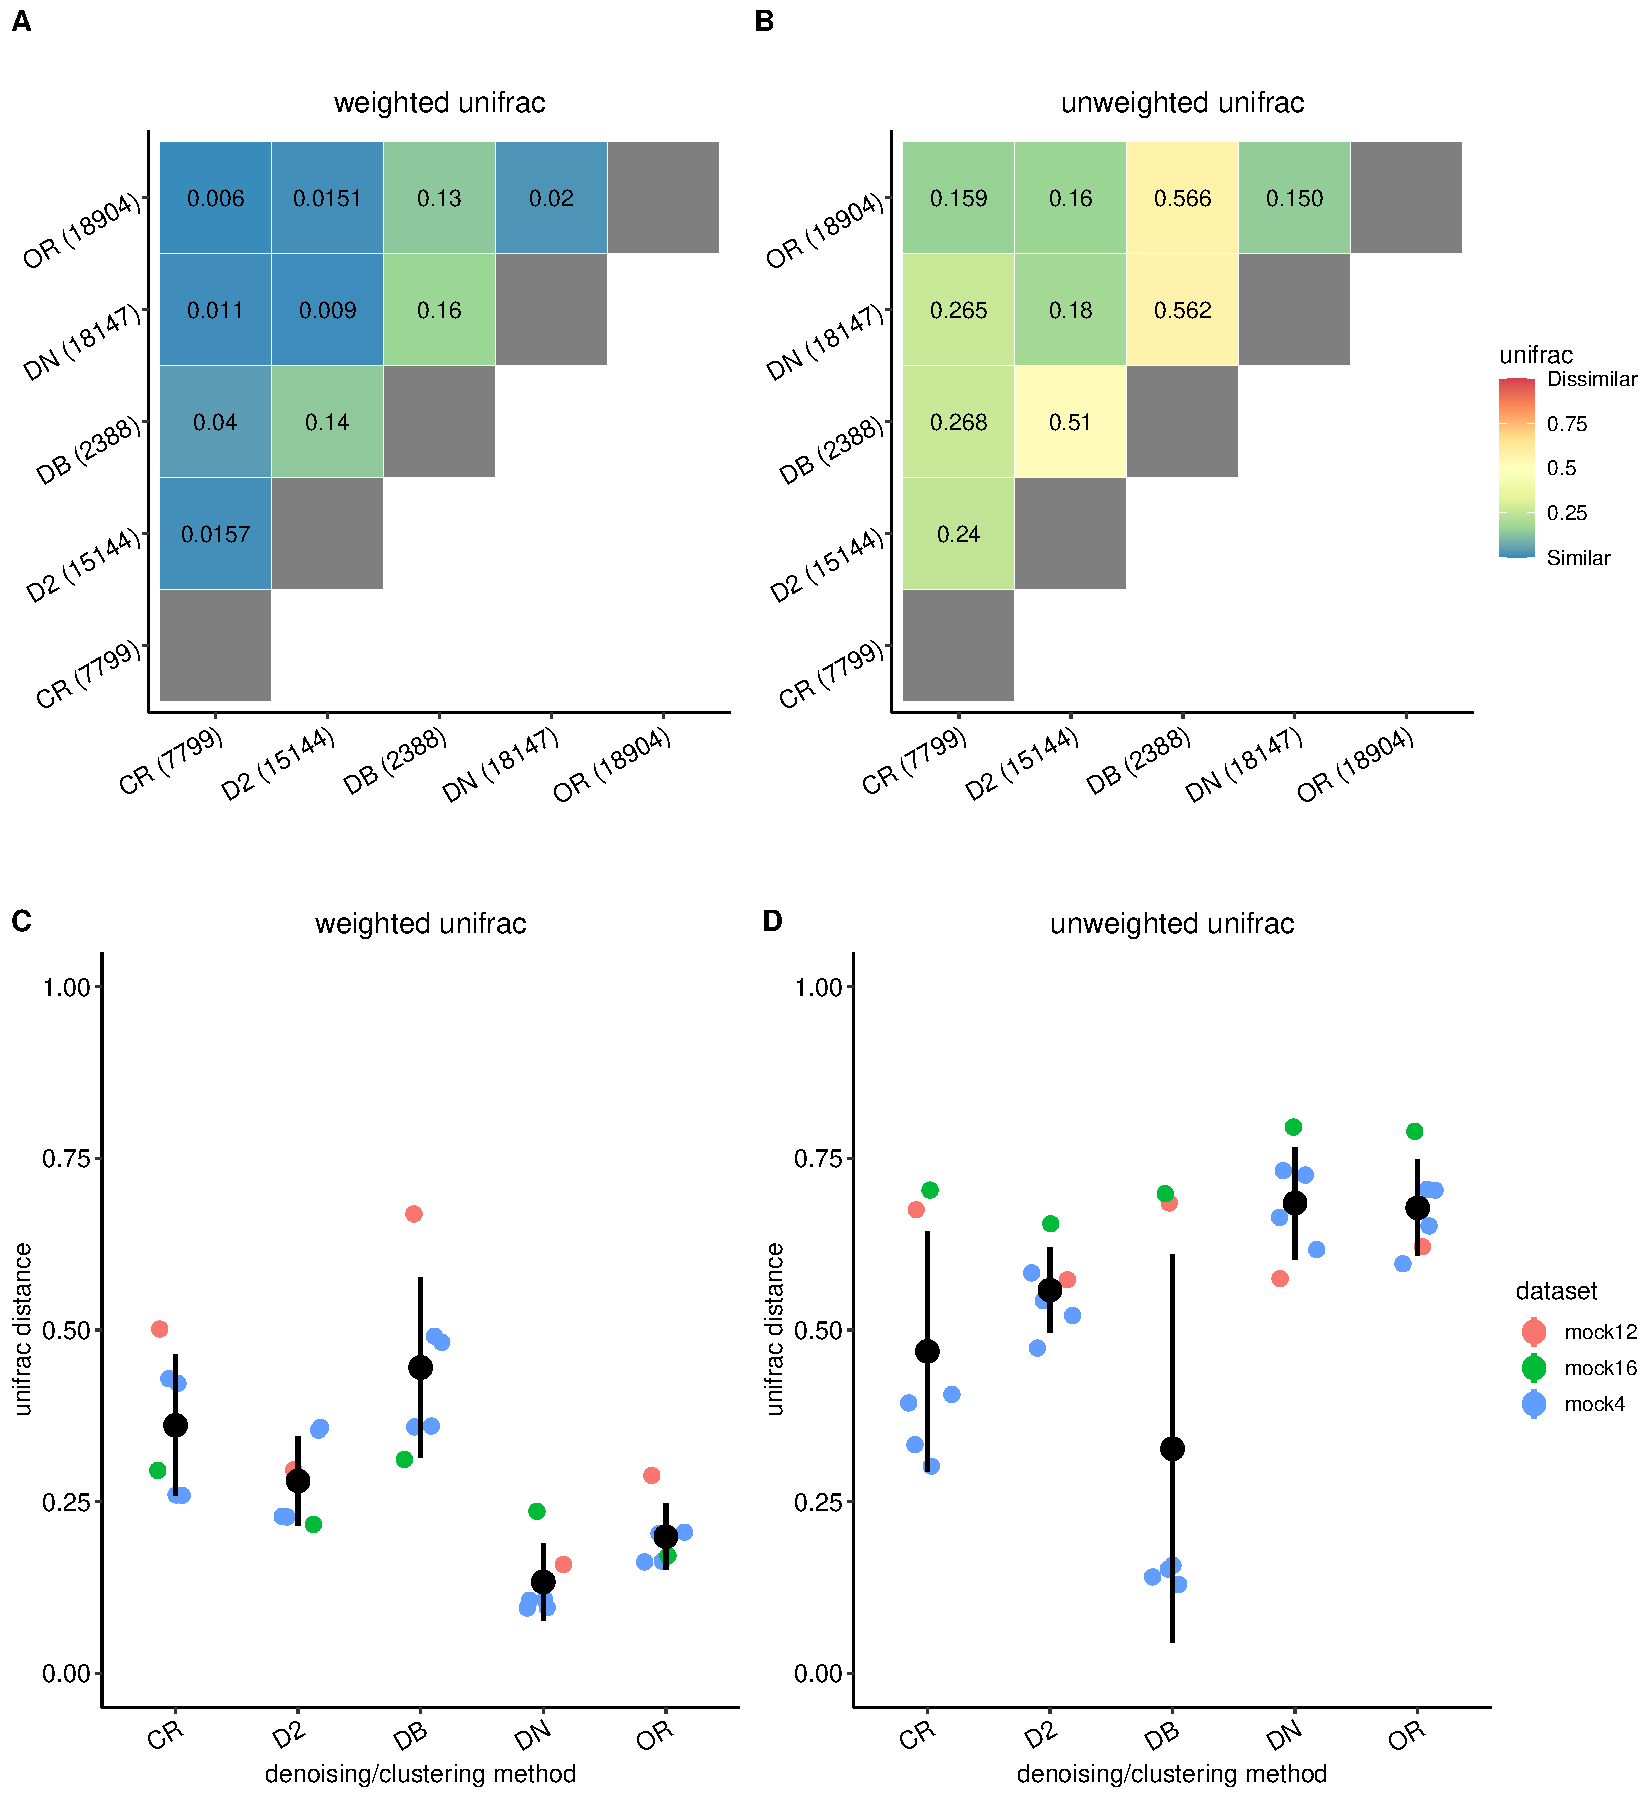
\includegraphics[width=\textwidth]{figure3.pdf}
    \caption{
      \textbf{The representative sequences generated by the different denoising/clustering methods are very similar but differ in the sequences that are in low abundance.}
      \textbf{(A)} The average weighted UniFrac distance between the representative sequences shows that the representative sequences and their compositions are fairly identical between the methods,
      \textbf{(B)} The relatively larger average unweighted UniFrac distance indicates that methods differ in their identification of sequences of low abundance,
      \textbf{(C, D)} The distributions of the avegage weighted UniFrac distance between the expected sequence profile and the calculated sequence profile in mock datasets.
      \textbf{(D)} The distributions of the average unweighted UniFrac distance show that dada2 and Deblur were the best performing methods in most of the datasets.
    }
    \label{fig:figure3}
  \end{figure}

  \FloatBarrier

  \subsection*{Taxonomy databases vary widely in taxonomy hierarchy and update frequency}

  Taxonomy databases are used to assign taxonomic identities to the representative sequences obtained after the DC step.
  In order to compare the assigned taxonomies from different databases, we use the same reference sequences and assign taxonomies to them using different taxonomy reference databases.
  The three 16S taxonomic reference databases used in this study are SILVA~\cite{Quast2012}, \ac{gg}~\cite{DeSantis2006} and \ac{ncbi} RefSeq.
  SILVA and \ac{gg} are two popular 16S databases used for taxonomy identification.
  The \ac{ncbi} RefSeq nucleotide database contains 16S rRNA sequences as a part of two BioProjects - 33175 and 33317.
  The three databases vastly differ in terms of their last update status - \ac{gg} was last updated on May 2013, SILVA was last updated on December 2017 at the time of writing and \ac{ncbi} is updated as new sequences are curated.
  Since updates to taxonomic classifications are frequent, these databases vary significantly in terms of taxonomy hierarchies~\cite{Balvociute2017}.

  The representative sequences obtained from the \ac{dada2} method in DC step were used for taxonomic assignment using the three reference databases.
  Figure~\ref{fig:figure4}A depicts a flow diagram that shows how the top 50 representative sequences (sorted by abundance) are assigned a Genus according to the three different databases.
  We observe that not only does the assigned Genus composition vary significantly, but the percentage of unassigned representative sequences (gray) also differ.
  Even the most abundant representative sequence is assigned to an "unknown" Genus in two of the three databases.
  A representative sequence might be assigned an "unknown" Genus for one of two reasons: the first is if the taxonomy identifier associated with the sequence in the database did not contain a Genus; the second (more likely) reason is that the database contains multiple sequences that are very similar to the query (representative) sequence and the consensus algorithm (from \ac{qiime2}) is unable to assign one particular Genus at the required confidence.
  After assigning all the representative sequences to taxonomies we perform a pairwise comparison of the similarity between assignments from different databases at every taxonomic level (Figure~\ref{fig:figure4}B).
  The assignments beyond Family level (Family, Genus and Species) are very dissimilar with $<70\%$ similarity between any pair of databases.
  There are no two reference databases that are more similar than the other, with \ac{gg} and SILVA producing only marginally similar assignments compared to \ac{ncbi}.
  This implies that the taxonomy assignments from each reference database are fairly unique and is one of the reasons for a large differences in the resultant co-occurrence networks generated from different taxonomy databases.
   % TODO: Update this
  Supplementary Figure~\ref{fig:figureS4} shows that the top 20 most abundant genera in the three resulting taxonomy composition tables are different.
  For example, the most abundant genus in the \ac{gg} taxonomy table was \textit{Escherichia} whereas in the SILVA taxonomy table it was \textit{Escherichia-Shigella}.
  Although these are minor differences, when comparing a large number of taxonomy composition tables these problems are hard to diagnose.
%   The comparison of all assigned genera instead of the just the top 20 contains the same percentage of matches and mismatches, implying that there does not seem to exist a correlation between abundance and mismatch.
%   This suggests that the most abundant sequences are not necessarily the ones that are consistently matched to the same taxonomies in the different reference databases.

  As in the previous section, these comparisons only indicate similarity or dissimilarity between methods.
  In order to obtain an absolute measure of accuracy of the taxonomic assignments we use the expected reference sequences from the mock datasets as the query sequences for the databases and the expected taxonomic composition as the standard to compare against (Figure~\ref{fig:figure4}C).
  Again, we observe that none of the databases perform better than the others in absolute terms.

  Given that no database performs better than others against mock datasets, and that databases are almost equally distant from each other in terms of final output, the choice of which database to use should be driven by other reason. One user-specific way to choose, would be based on the known representation of taxa for the microbiome of interest (see also Discussion). Another reason could be the frequency of updates and the potential for future growth, which prompted us to set \ac{ncbi} as the \ac{micone} standard for taxonomy assignment.
 In addition to being regularly maintained and updated the \ac{ncbi} database has the advantage that its accuracy of assignments is still comparable to the SILVA and \ac{gg} reference databases that are routinely used as reference databases.

  \begin{figure}[H]
    \centering
    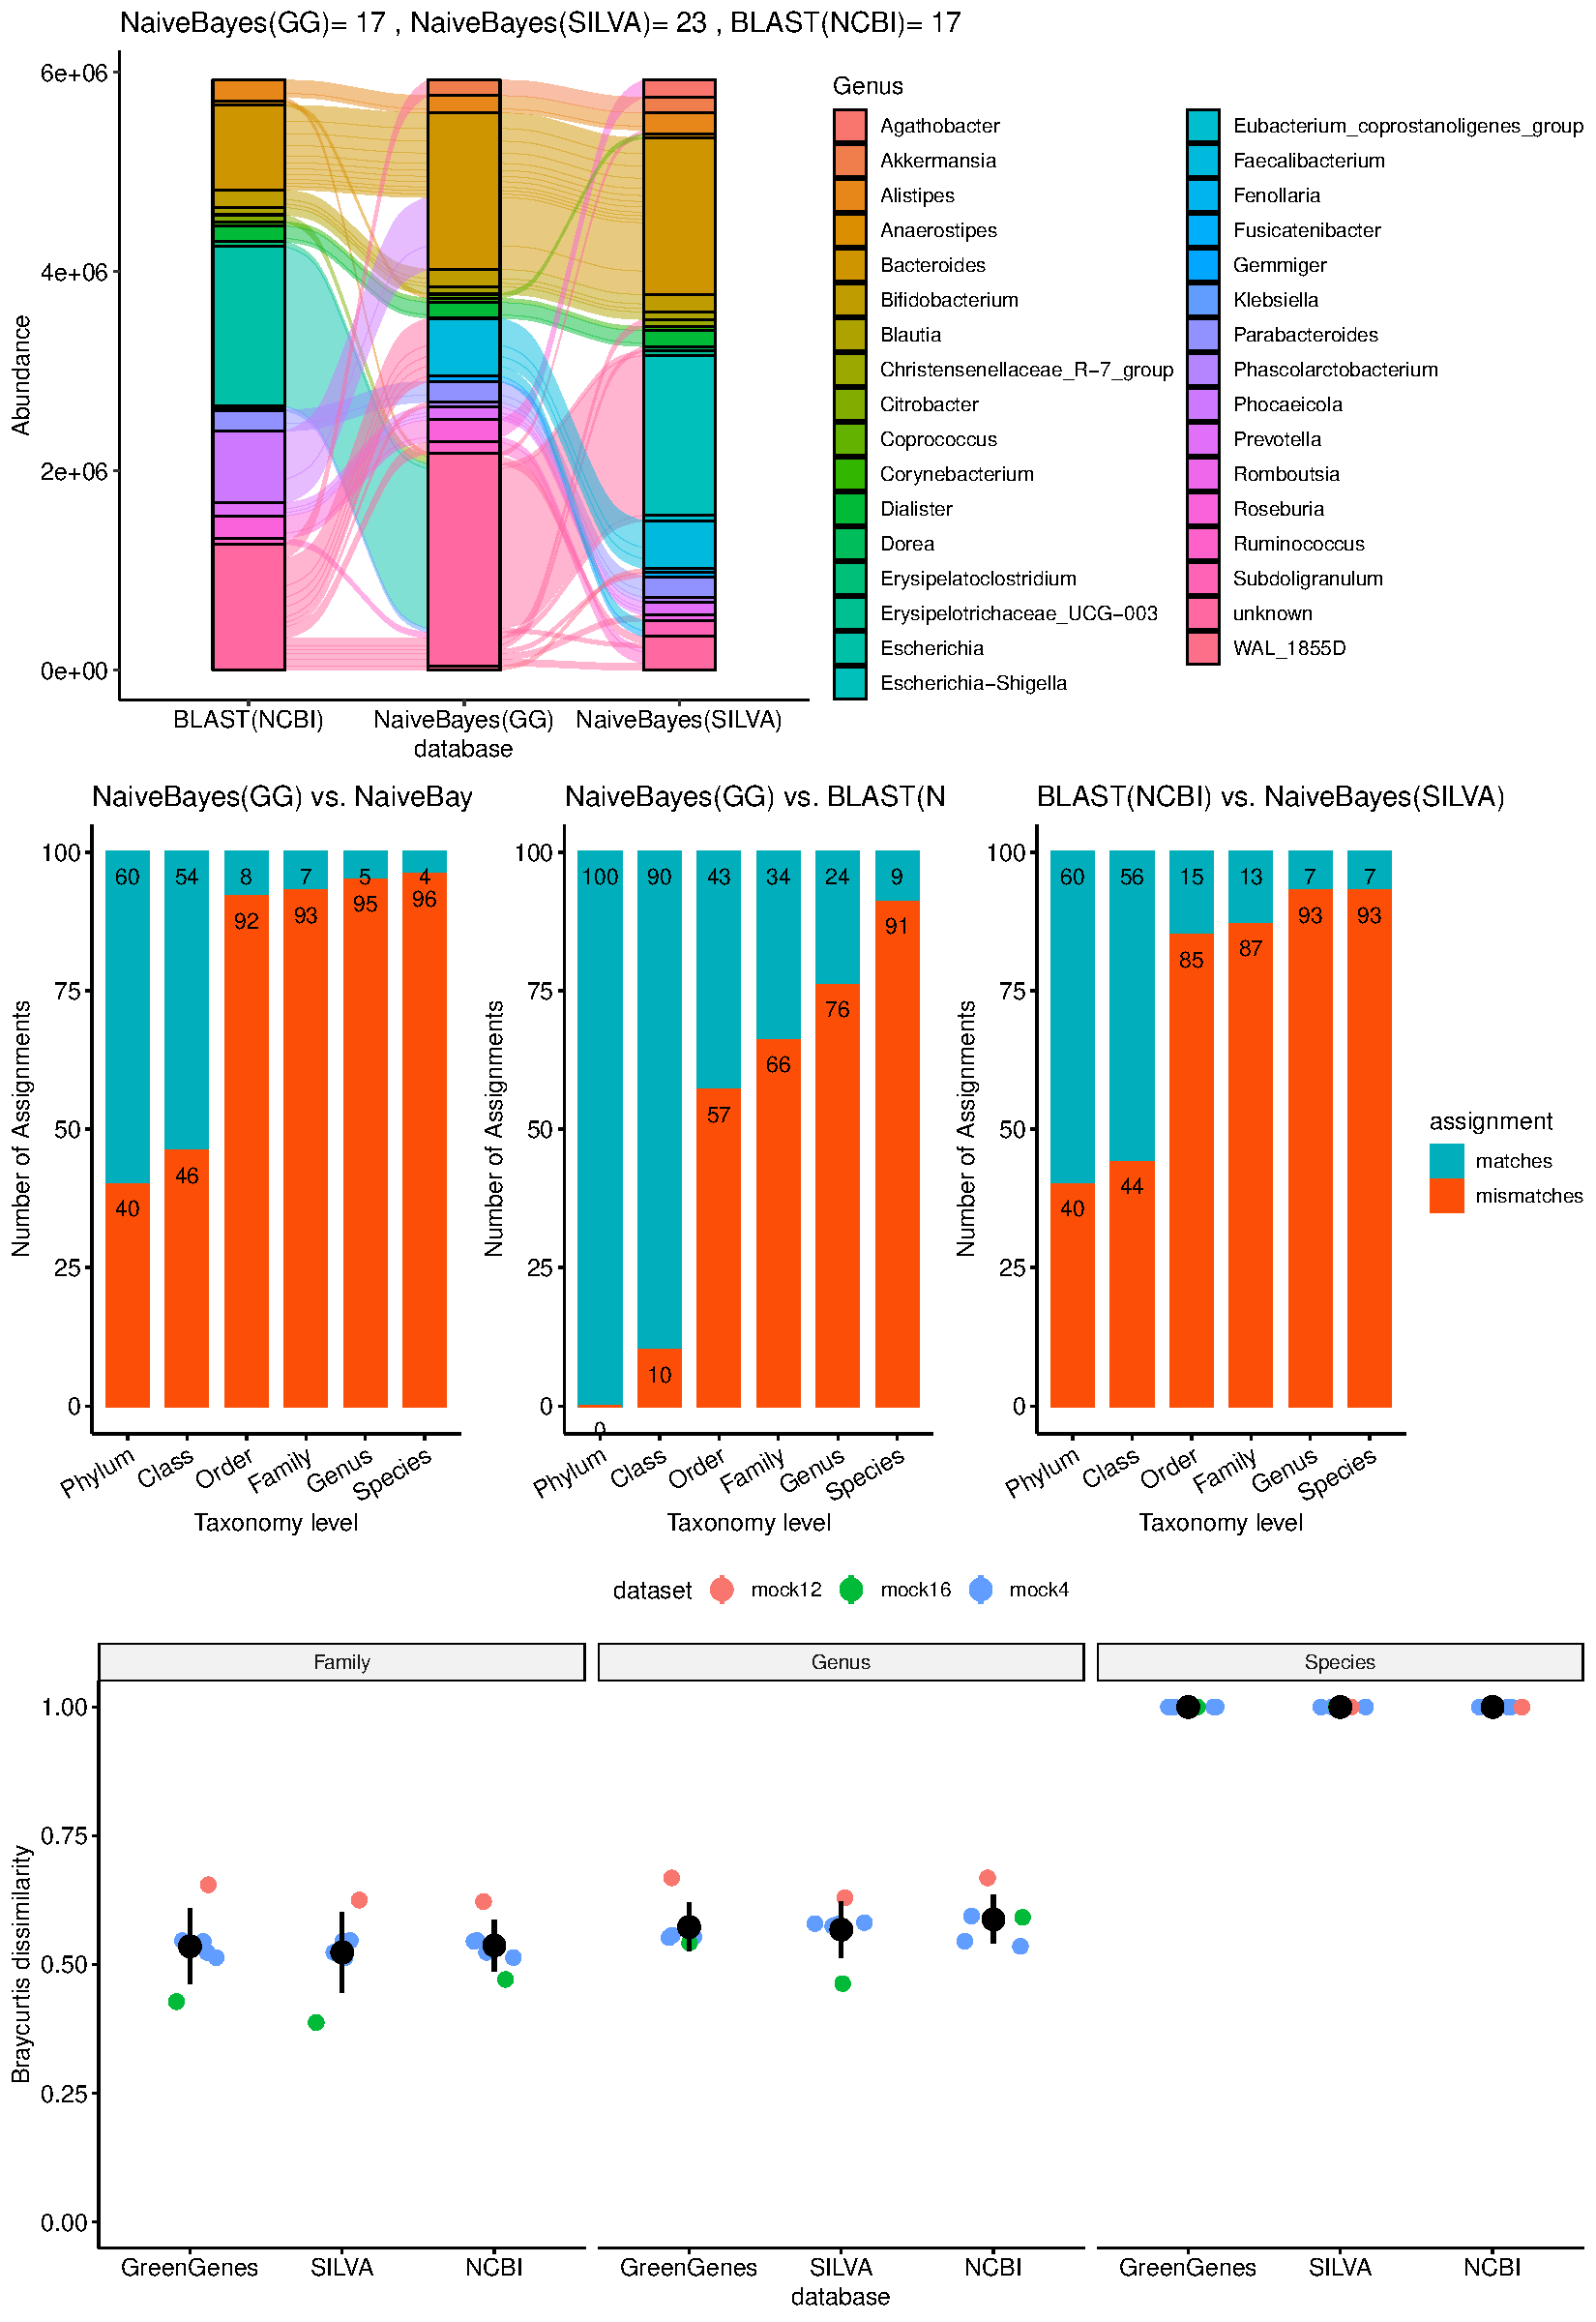
\includegraphics[width=0.9\textwidth,height=1.2\textwidth]{figure4.pdf}
  \end{figure}
  \begin{figure}[!t]
    \centering
    \caption{
      \textbf{Taxonomic reference databases vary widely in terms of their taxonomy assignments.}
      \textbf{(A)} The assignment of the top 50 representative sequences to their respective taxonomies using the three different reference databases shows how the same sequences are assigned to different Genus.
      \textbf{(B)} The percentage of \ac{otu}s assigned to the same taxonomic label when using different reference databases.
      The percentage of mismatches decrease at higher taxonomic levels but even at the Phylum level there exists around 10\% of mismatches.
      \textbf{(C)} The Bray-Curtis dissimilarity between the expected taxonomy profile and calculated taxonomy profile in the mock datasets shows that there is no singular best choice of database for every dataset.
    }
    \label{fig:figure4}
  \end{figure}

    

  \FloatBarrier

  \subsection*{Networks generated using different network inference methods show notable difference in edge-density and connectivity}

  % TODO: Talk about the difference between correlations and associations
  The six different network inference methods used in this study are \ac{magma}~\hl{in biorxiv [ADD REF]}, \ac{mldm}~\cite{Yang2017}, \ac{spieceasi}~\cite{Kurtz2015}, \ac{sparcc}~\cite{Friedman2012}, Spearman and Pearson.
  These network inference methods into two groups, the first set of methods (Pearson, Spearman, \ac{sparcc}) infer pairwise correlations while the second set infer direct associations (\ac{spieceasi}, \ac{mldm}, \ac{magma}).

  For the analysis presented in this section, we used the taxonomy composition table obtained using the \ac{ncbi} reference database as the input for algorithms that infer co-occurrence associations between the microbes.
  Figure~\ref{fig:figure5}A shows the networks inferred from this dataset using the different inference algorithms.
  We can clearly see that the different networks differ vastly in their edge-density and connectivity and even some of the edges in common to these networks have their signs inverted. Note, however, that some of these comparisons depend on the threshold that has to be applied to the pairwise correlations methods (currently 0.3, based on [REF]).
  To get a more quantitative idea, we can take a look at the nodes and edges (Figure~\ref{fig:figure5}B) in common between the networks using UpSet plots (only \ac{magma}, \ac{mldm}, \ac{spieceasi}, \ac{sparcc} are used in the comparison).
  The results for the node intersections show that the networks have a large number of nodes in common ($63$ out of $67$ nodes in the smallest network - \ac{magma}) and no network possesses any unique node.
  The edge intersections in contrast show that only $19$ edges (out of $98$ edges in the smallest network - \ac{magma}) are in common between all the methods and each network has a large number of unique edges.
  These results indicate that there is a substantial rewiring of connections in the inferred networks.

  Unlike in the previous sections, where were we evaluated the performance of methods on mock datasets, there are no such datasets that contain a set of known interactions for the evaluation of the network inference algorithms.
  Therefore, we propose the construction of a consensus network (Figure~\ref{fig:figure5}C) involving \ac{magma}, \ac{mldm}, \ac{spieceasi} and \ac{sparcc} by merging the p-values generated from bootstraps of the original taxonomy composition table using the Browns p-value combining method [ref] (see Methods section).
  Based on this approach, \ac{micone} reports as default output the consensus network, annotated with weights (correlations for \ac{sparcc} and direct associations for the other methods) for all four methods.

  \begin{figure}[H]
    \centering
    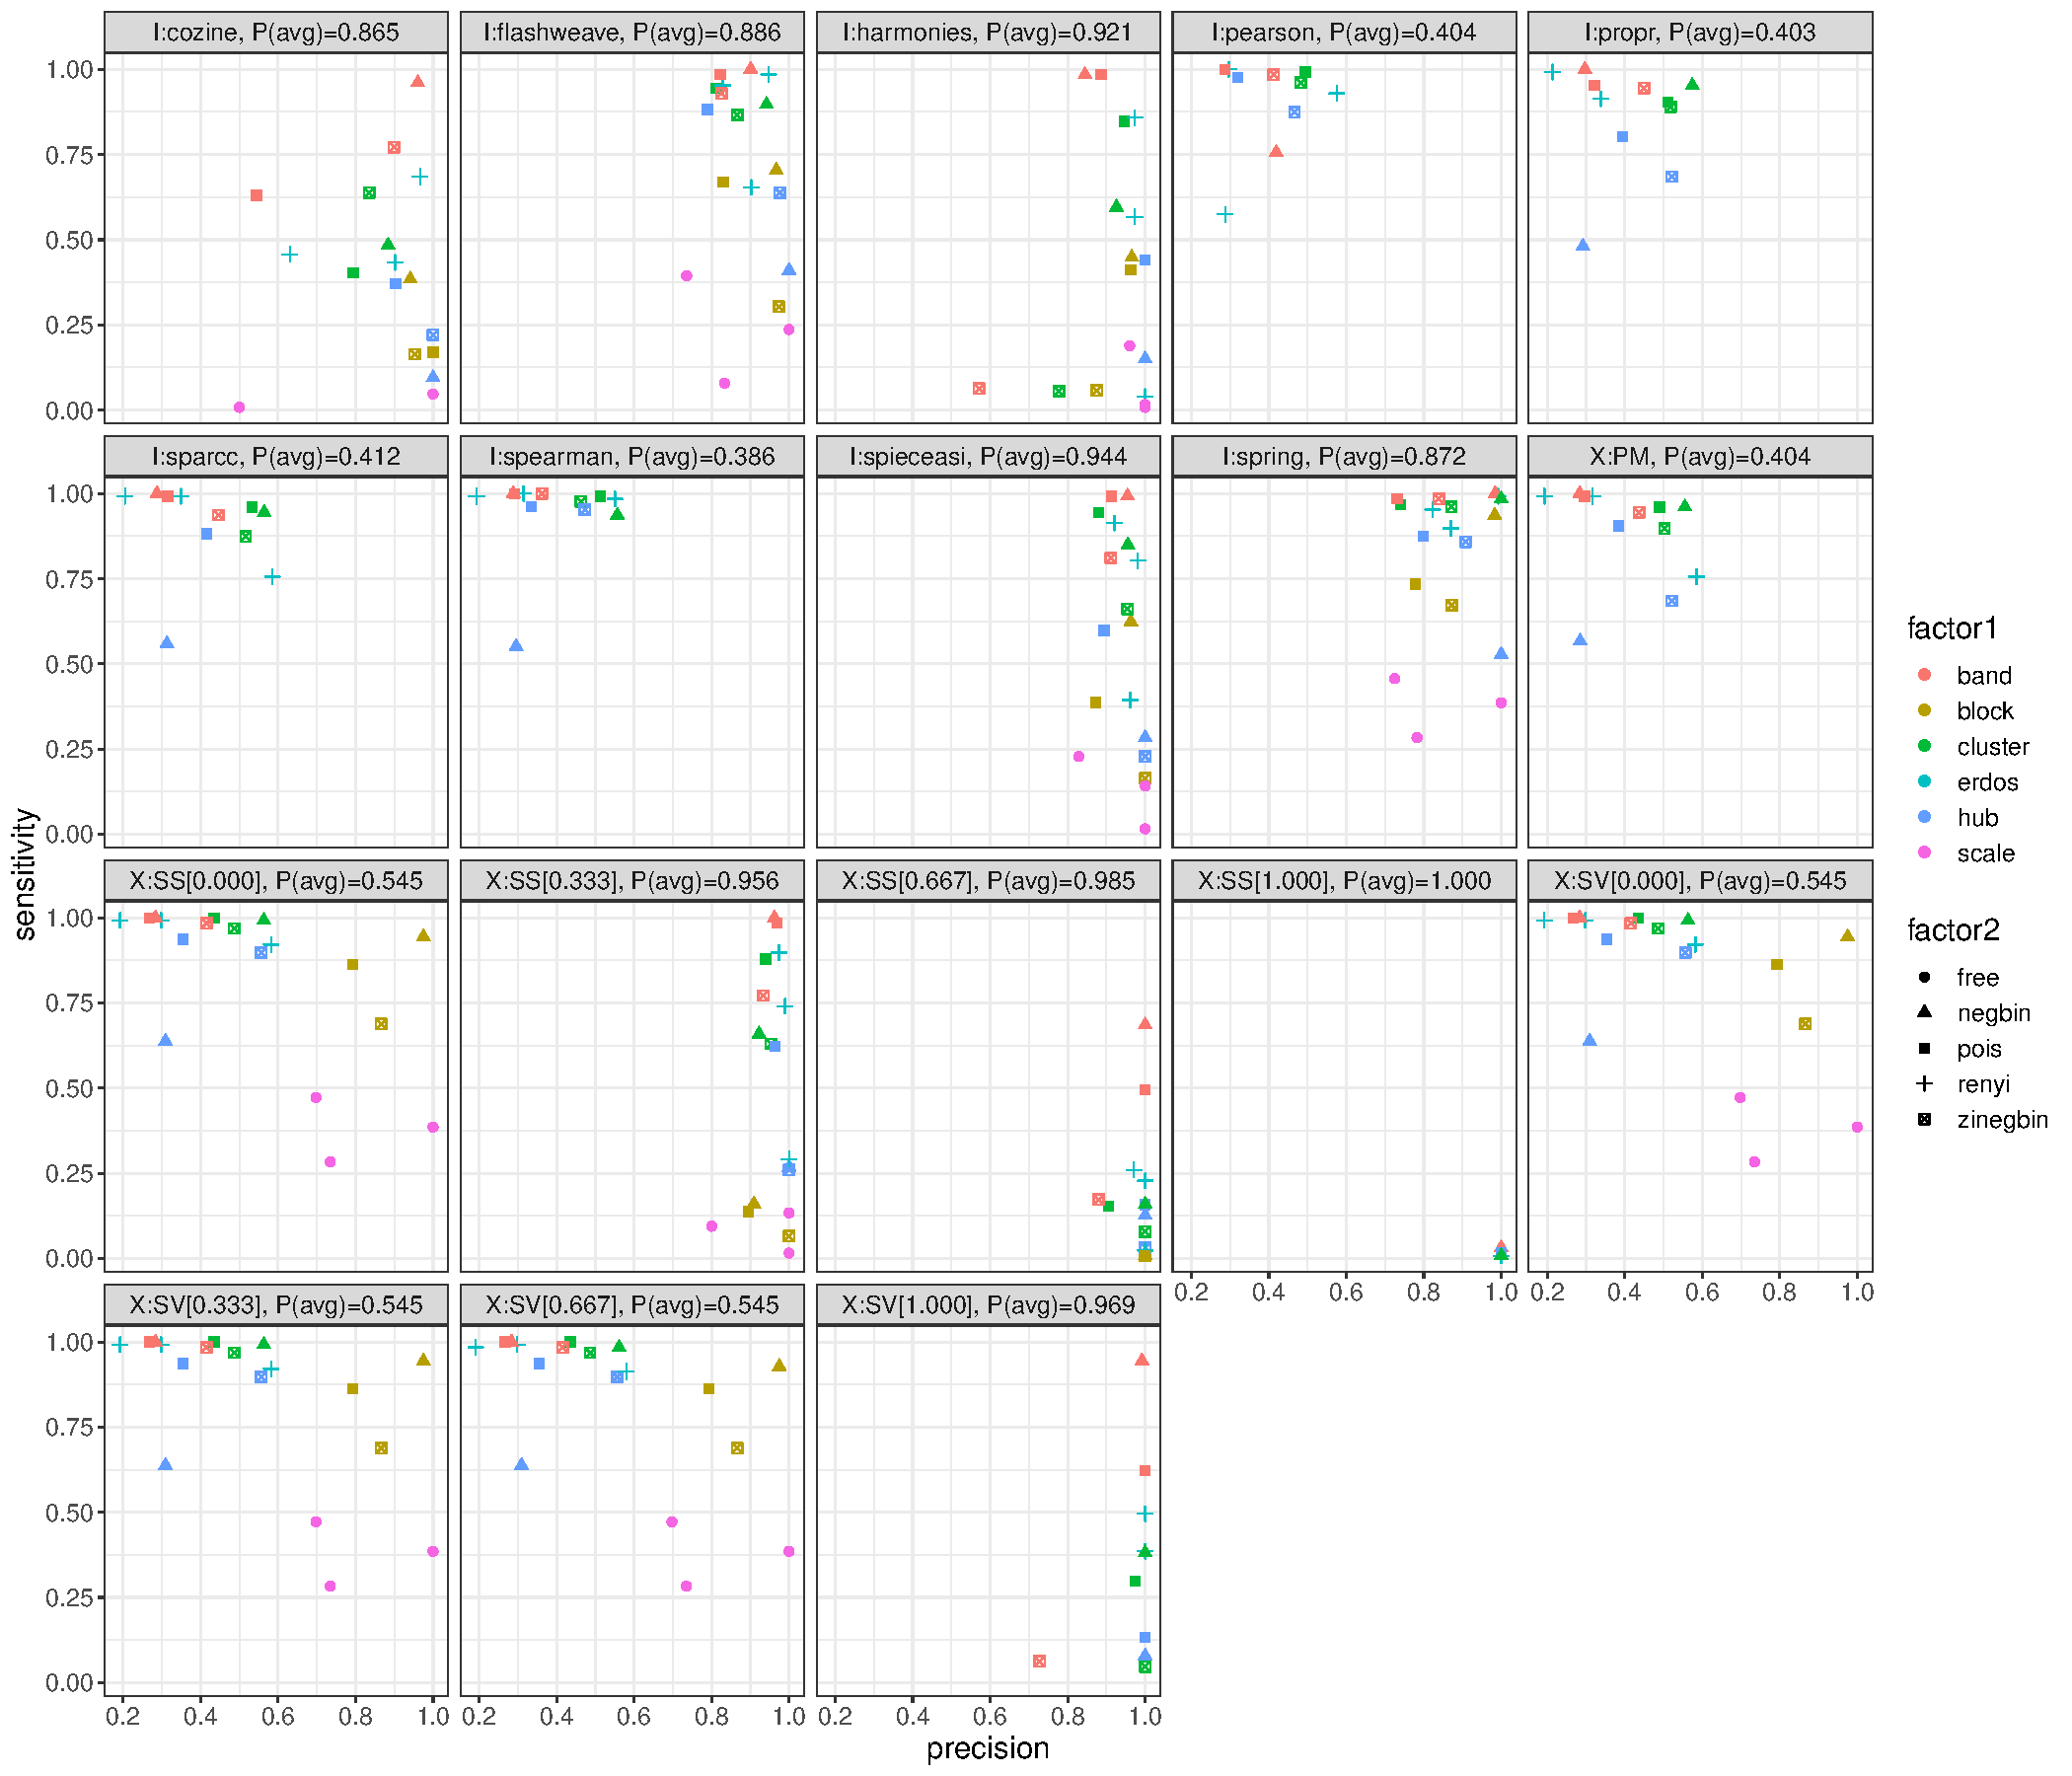
\includegraphics[width=0.9\textwidth]{figure5.pdf}
  \end{figure}
  \begin{figure}[t!]
    \centering
    \caption{
      \textbf{Networks generated using different network inference methods show notable differences both in terms of edge-density and connectivity}.
      \textbf{(A)} The six different networks generated by the different network inference methods are very dissimilar.
      The green links are positive associations and the orange links are negative associations.
      A threshold of 0.3 was set for the methods that infer pairwise correlations (\ac{sparcc}, Spearman, Pearson) and no threshold was set for the other methods.
      \textbf{(B)} The node overlap upset plot indicates that all the networks have a large number of common nodes involved in connections.
      Whereas, \textbf{(C)} The edge overlap upset plot shows that a very small fraction of these connections are actually shared.
    }
    \label{fig:figure5}
  \end{figure}

 

  \FloatBarrier

  \subsubsection*{The default pipeline}
  
  The systematic analyses performed in the previous sections clearly show that the choice of tools and parameters can have a big impact on the final co-occurrence network. For some of these choices (e.g. \ac{dada2} vs. deblur) there is no clear metric to establish a best protocol.
  For other choices, the mock communities provide an opportunity to select combination of parameters that yield more accurate and robust results.
  Despite this partial degree of assessment, we wish to suggest a combination of tools and parameters that produce networks that are derived from the combination of tools which performed best on the mock communities, and displayed highest robustness to switching to alternative methods.
  These tools and parameters are chosen as the defaults for the pipeline and are given in Table~\ref{tab:default_options}.

  \begin{table}[h]
    \centering
    \small
    \begin{tabular}{|c|c|c|}
      \hline
      \textbf{Process} & \textbf{Tool} & \textbf{Parameters} \\
      \hline
      Denoising and Clustering & Dada2/Deblur & default \\
      Taxonomy Assignment & \ac{ncbi} with Blast & RefSeq database \\
      OTU Processing & Based on statistical power & Dynamic cutoff \\
      Network Inference & Consensus method & - \\
      \hline
    \end{tabular}
    \caption{Default tools and parameters for the pipeline}
    \label{tab:default_options}
  \end{table}

  The recommended tool for the \ac{dc} step (\ac{dada2} or Deblur) were chosen based on their accuracy in recapitulating the reference sequences in mock communities and synthetic data.
  The choice of the taxonomy reference database in the \ac{ta} step is dictated largely by the species expected to be present in the sample as well the database used in similar studies if comparison is a goal.
  Nevertheless, we suggest \ac{ncbi} RefSeq along with blast+ as the query tool since the database is updated regularly and has a broad collection of taxonomies.
  The abundance threshold at the \ac{op} step is determined automatically based on the number of samples and the required statistical power.
  Finally, we use the Browns p-value combining method on the networks generated using \ac{magma}, \ac{mldm}, \ac{spieceasi} and \ac{sparcc} to obtain a final consensus network in the \ac{ni} step.

  Figure~\ref{fig:figure6}A shows the default network compared against networks generated by altering one of the steps of the pipeline from the default.
  These results indicate that the biggest differences in networks occur when the reference database or the network inference algorithm are changed.
  Furthermore, the L1 distance of networks generated by altering one of the steps of the pipeline from the default against the default network (Figure~\ref{fig:figure6}B) shows that the biggest deviations from the default network occur when the \ac{ta} and \ac{ni} steps are changed, reinforcing the same results observed in Figure~\ref{fig:figure2}. Figure~\ref{fig:figure7} shows the co-occurrence networks inferred for the hard palate for healthy subjects in a periodontal disease study~\cite{Chen2018} and the healthy stool microbiome in fecal microbial transplant study~\cite{Kang2017}. These consensus networks were generated using the default tools and parameters from Table~\ref{tab:default_options}.

  \begin{figure}[h]
    \centering
    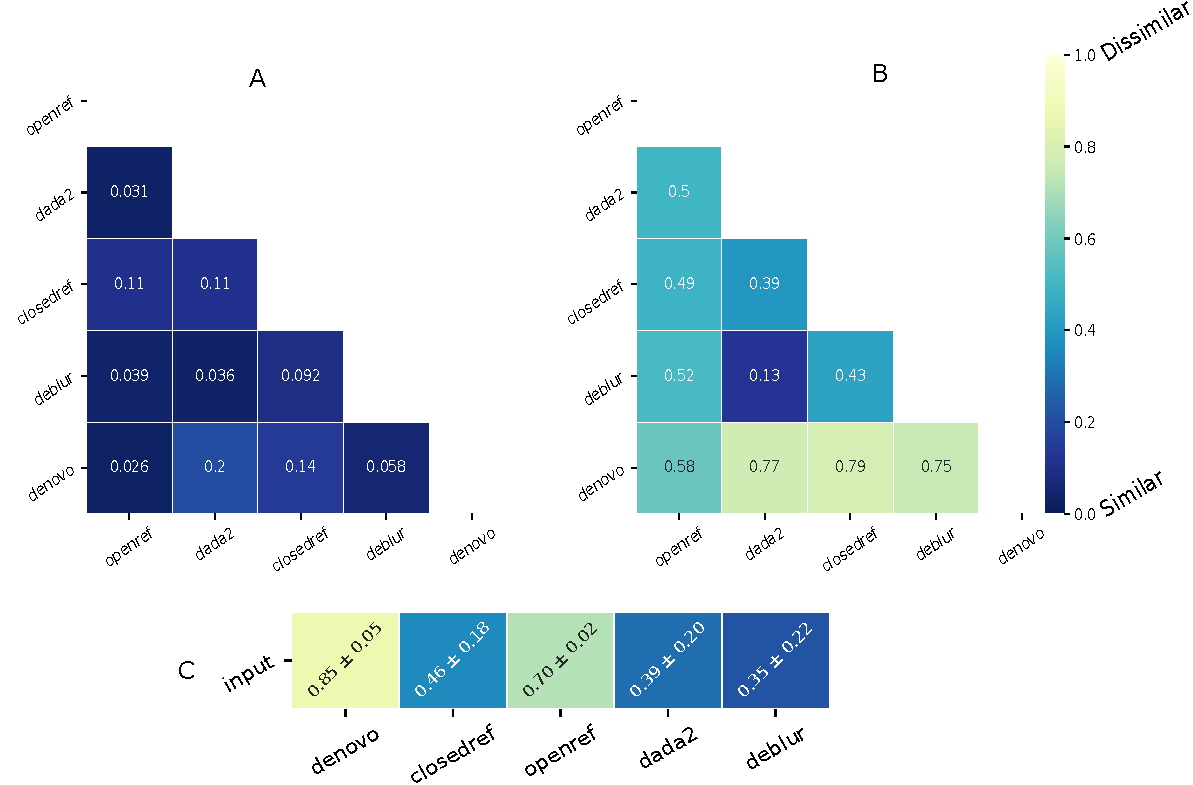
\includegraphics[width=0.85\linewidth]{figure6.pdf}
    \caption{
      \textbf{Network inference and taxonomic assignment have the highest influence on the inferred network structures.}
      \textbf{(A)} The network constructed using the default pipeline parameters (DC=\ac{dada2}, TA=\ac{ncbi}, OP=on, NI=\ac{sparcc}) is compared with networks generated when one of the steps use a different tool.
      The common connections (common with the default network) are in black, connections unique to the network are colored purple and connections in the default network but not present in the current network are gray.
      \textbf{(B)} The L1 distance between the networks generated by changing one step of the default pipeline and the network generated using the default parameters.
    }
    \label{fig:figure6}
  \end{figure}


  \begin{figure}[h]
    \centering
    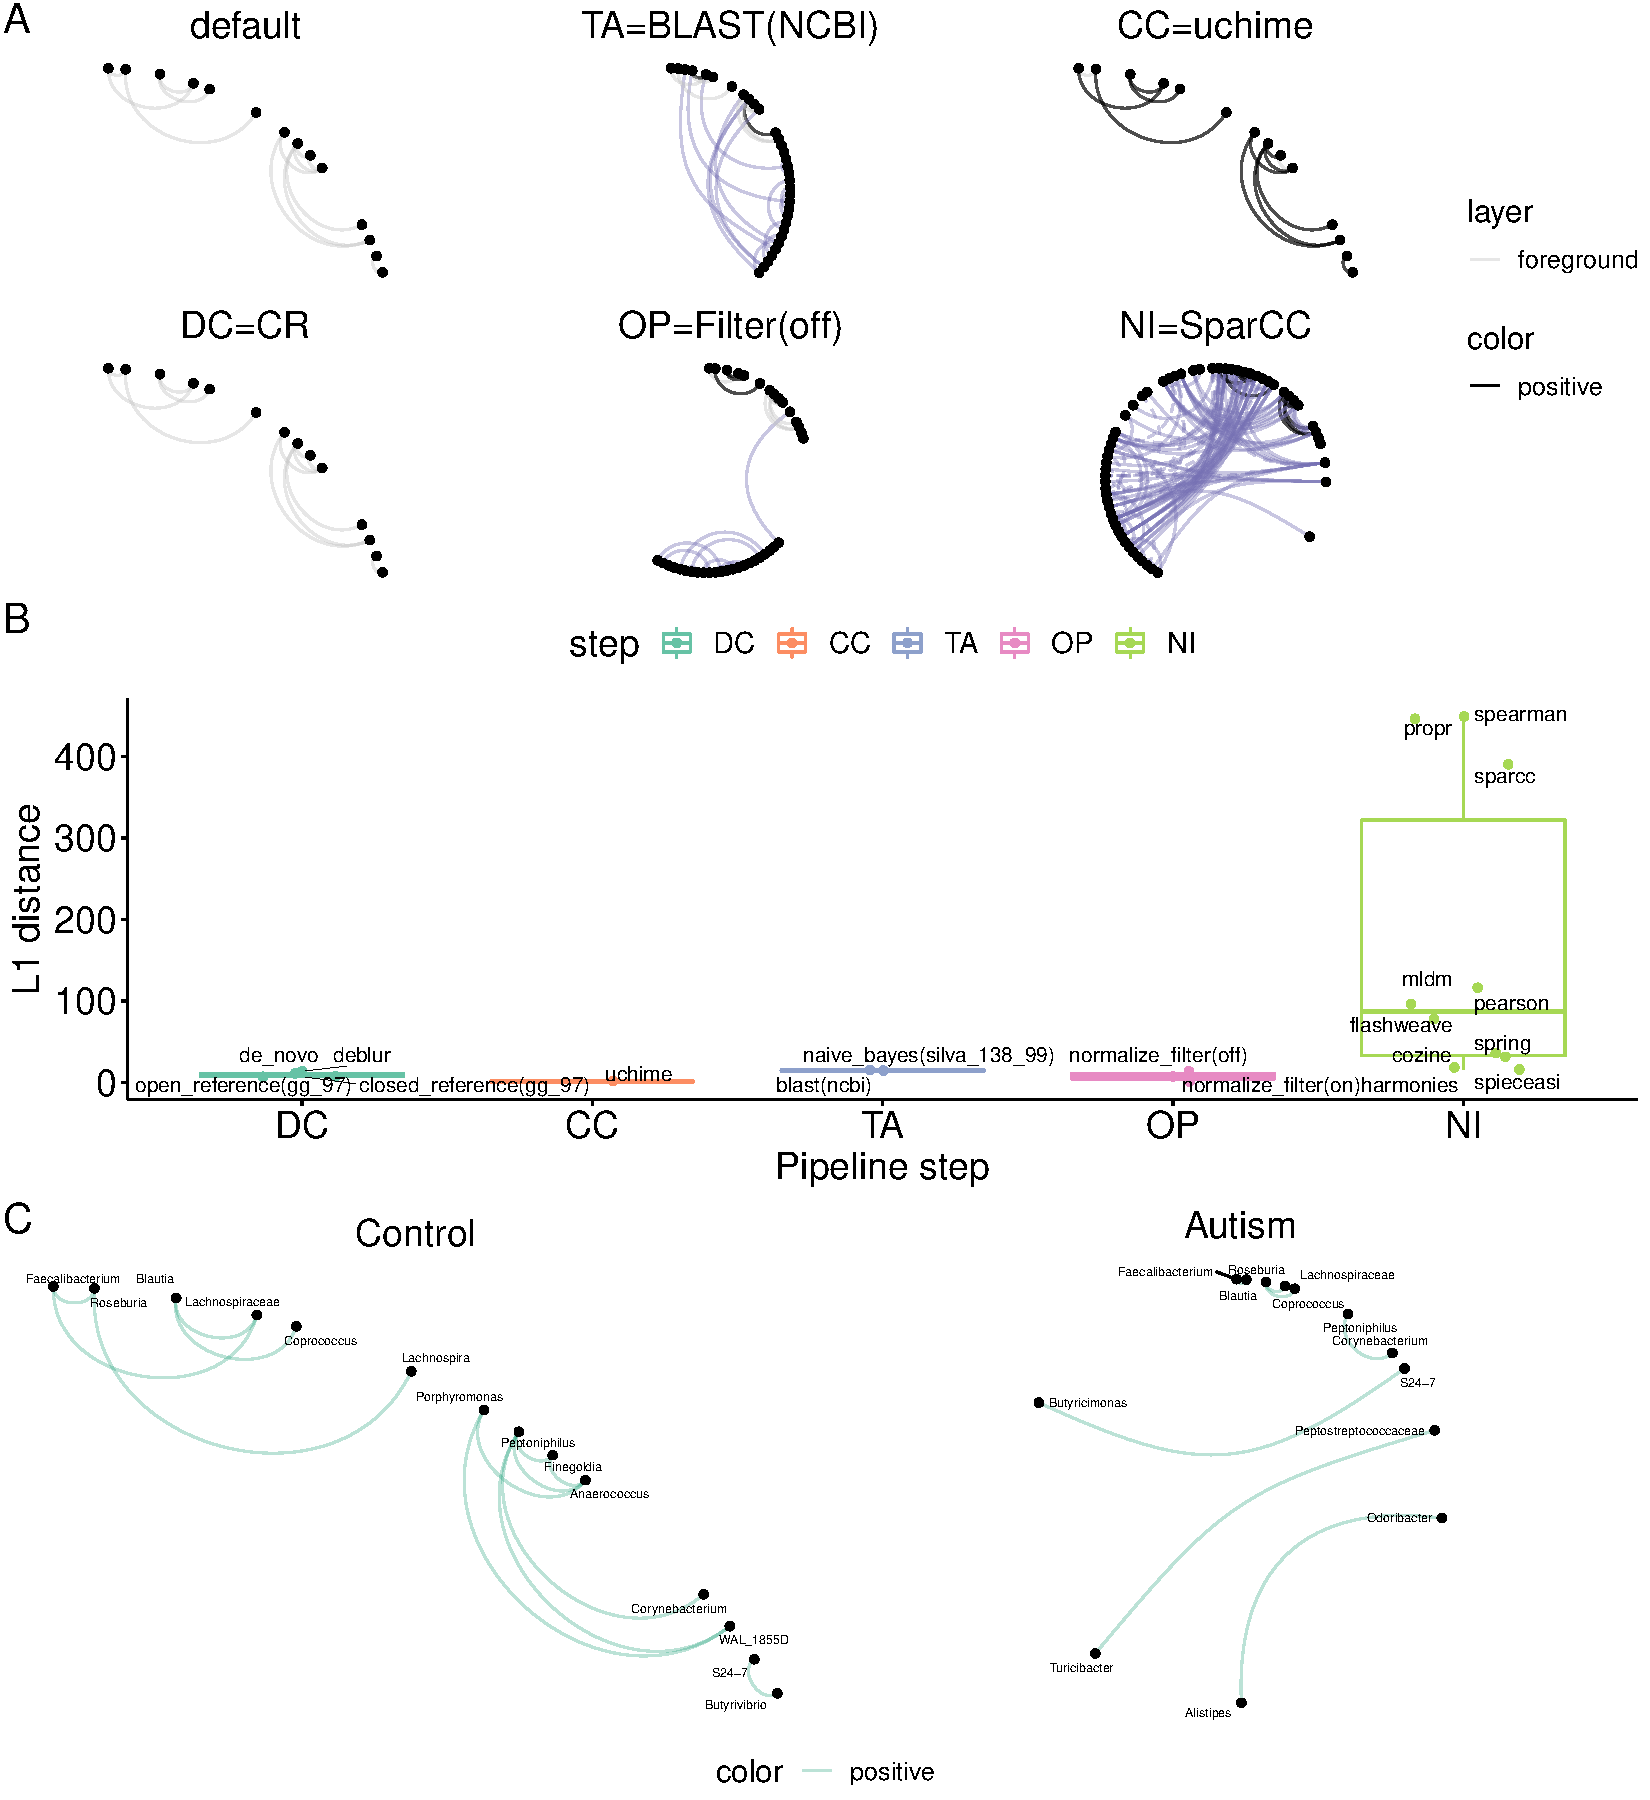
\includegraphics[width=17cm]{figure7.pdf}
    \caption{
      The consensus networks generated using the default pipeline settings.
      \textbf{(A)} Co-occurrence network of the Hard Palate microbiome generated from samples of healthy subjects in a periodontal diseases study.
      \textbf{(B)} Co-occurrence network of the Stool microbiome generated from samples of healthy subjects in a fecal microbiome transplant study.
  }
    \label{fig:figure7}
  \end{figure}
